\chapter{Business context}
\label{chap:business-context}


A Supply Chain is a system of organizations, people, activities, information, and resources involved in moving a product or service from supplier to customer.
Its activities extends from the recovery of raw material to their transformation into finished product and their delivery to the costumer.


\section{Supply Chain objectives}


Satisfaction clients is based on a trade-off between low cost, appropriate and quality product or service and short delivery lead time.
To reach this optimum, \ie be competitive, companies and their Supply Chain must face many objectives often contradictory.
%Because resources are finite and because of the wide variety of its activities, Supply Chain faces many objectives sometimes contradictory. 
They can be classified in three categories.
\begin{itemize}
  \item \emph{Costs.} Classic examples are production costs (purchase of plants, warehouse or machines, salaries) or shipping costs (regardless of transportation mode, of rental or purchase).
  \emph{Flexibility}, which is the ability to face variations of the products mix, or \emph{capacitative reactivity}, which is the ability to face variations on the global volume, are also costs since it implies investments.

  \item \emph{Stocks.} Even if it looks like a cost, stocks have their own characteristics.
  They correspond to working capital and they cannot be compared to industrial costs.

  \item \emph{Service.} It measures the ability of Supply Chain to deliver the right product with respect to deadlines.
\end{itemize}
In an ideal case, cost and stock must be very low whereas service must be very high.
However, it is easy to see the contradictions.
In automotive industry, high stock is impossible because of depreciation an diversity of products.
However, service level must be high which implies a huge flexibility.
In luxury industry, availability of the right product in the right store is more critical than manufacturing cost.
Among other examples, over-capacity increases flexibility but is expensive or specialization of assembly lines or plants increases productivity but often reduces flexibility.
Depending on the industry, a trade-off between these three incomparable quantities must be found.
The decision-maker must define which one is the objective and which ones are constraints or simply ignored.



\section{Presentation of Argon Consulting}


Argon Consulting is an international, independent consulting firm whose mission is to help its clients achieve sustainable competitive advantage through operational excellence.
It begin its consultancy activity in 2001 and employs over 230 consultants in six offices: Paris, London, Atlanta, Singapore, Melbourne and Mumbai.


Argon consulting have assisted many companies in operational transformation projects (R\&D, Procurement, Manufacturing, Supply Chain, Distribution, Services, SG\&A, Performance Management, Change Management).
Industries served cover
\emph{Aerospace \& Defense} (Lat\'eco\`ere, Safran, Thales) and
\emph{Discrete Manufacturing} (Alstom, SNCF, DCNS) which have small-series and large program logic as well as
\emph{Retail} (ADEO, Carrefour, Cdiscount) which sells products or services to large number of customers through multiple channels of distribution.
In the mid of these extremes, we also find
\emph{Automotive} (Michelin, PSA, Valeo) where innovation performance and diversity of products is challenging,
\emph{Consumer Packaged Goods} (Bel, Danone, L'Oréal) where decreasing consumption and fluctuation of productions costs reduce profitability and
\emph{Textile} (Galeries Lafayette, Cama\"ieu, Kiabi) where fast product renewal and fast evolution of sourcing is critical at operational level.
Among other sectors with specific rules,
\emph{Luxury Goods} has highly erratic demand and is extremely competitive,
\emph{Pharmaceutical Industry} (Merck, Sanofi, Servier) has economic pressure applied by state authorities due to imbalance of the health insurance systems and
\emph{Energy \& Utilities} (EDF, ENGIE) is capital-intensive, highly cyclical, fully globalized and at the heart of geostrategic issues.


Argon Consulting began as a consultancy company specialized in logistic.
Growing, it acquired expertise at every level of Supply Chain.
Argon Consulting describes itself as a multi-specialized firm whose competitive advantage comes from its ability to quantify their studies.
Through this thesis, the objective is to find a unified framework for some recurrent problems.
Moreover, Argon Consulting wants to scientifically tested the accuracy and efficiency of the models developed.



\section{Supply Chain organizations}


Supply Chain organizations can be classified into four main models \cite{arnold2007} which are represented in \cref{fig:supply-chain-models}.
Identify the best organization for an industry is critical to define which decisions are short-term, mid term or long-term and to know when costs, stock and service can be impacted.
\begin{itemize}
  \item \emph{Engineer-To-Order (ETO).}
  Client is involved in the design and gives engineering requirements and specifications which enables much customization and a specific design.
  The consequences are long delivery lead times due to purchasing of raw material and to designing.
  Classical domains are aeronautic or aerospace industries.

  \item \emph{Make-To-Order (MTO).}
  Products are made from standard items but with custom-designed components.
  Therefore, inventory are only composed of raw material and delivery lead time are still long.
  For example, marine energy turbines can be produced with a MTO organization.

  \item \emph{Assemble-To-Order (ATO).}
  Customer involvement is limited to selecting the component options.
  Thus, inventory are only composed of semi-finished products ready for assembly items and delivery lead time are short.
  Part of production of laptop follow this organization.

  \item \emph{Make-To-Stock (MTS).}
  Customer has very little involvement in the design.
  Products are engineered and manufactured to fill stocks which supplied clients demand.
  This organization enables the shortest delivery lead time.
  The majority of mass distribution products used this organization.
\end{itemize}


\begin{figure}[h]
  \centering
%  \includegraphics[width=\textwidth]{main/introduction/images/.tikz}
  \esgil{Include figure of the 5 supply chain models ou celle de la formation APICS (slide 4)}
  \caption{Exemple d'organisation de la Supply Chain d'un acteur du luxe}
  \label{fig:supply-chain-models}
\end{figure}



\section{Argon Consulting's clients cases}


Argon Consulting's application cases considered in this thesis are Assemble-To-Order and Make-To-Stock organizations.
We studied two applications in this thesis.
First one is mid-term and aims at minimize stocks.
Second one is long-term and aims at minimize industrial costs.


\subsection{Production planning}
\label{sec:business-context:argon:pdp}


This problem concerns directly the production function of the Supply Chain.
In Assemble-To-Order and Make-To-Stock organizations, inventory must be sufficient to serve demand at due date.
Then, production planning answers to both questions: when production starts and which quantity is produced.

Difficulties of this problem comes from many factors which prevent last minute production.
First, production capacities are limited.
Thus, production must be anticipated in order to deliver peak selling season, promotion program, vacation shutdown, etc.
It leads to inventory called \emph{anticipation inventory}.
Second, demand has random variations.
If demand or lead times are greater than forecast, a stock-out can occur.
To prevent it, a \emph{safety stock} is made.
Finally, \emph{flexibility} of means of production is limited.
Flexibility is the ability to change the item produced on a assembly line or in a plant.
Flexibility enables to face variations in the product mix.
Since it remains limited, \emph{lot-size inventories} also called \emph{cycle stocks} are needed. They are the portion of inventory that decreases gradually as customers’ orders come in and that are replenished cyclically when suppliers’ orders are received.


In Assemble-To-Order and Make-To-Stock production planning problems, stock is a main issue and decision-makers have a huge control on it.
Indeed, production decisions directly impacts inventory level.
Thus, its minimization is the objective of the problem.


Service level is a constraint.
In our applications, Argon Consulting's clients want to reach a service level.
This service level objective depends on the strategy of the company.
It was a trade-off between several objective as loss of reputation, intended costs, risk, benefits, etc.
For production planning problems, we take it as an input.
There are many indicators to measure service level.
A main distinction is between \emph{cycle service level} and \emph{fill rate service level}.
Cycle service corresponds to deliver a whole command at due date whereas fill rate service level measures the part of demand delivered at due date.
The choice depends on the industry.
Indeed, in case of complex products like in aeronautics, if one item is missing in the command, it can delayed the whole project.
Thus delivered the whole command is more important.
In case of simple products like in mass distribution, it more relevant to measure the part of demand delivered at due date.
Since we are interested in Assemble-To-Order and Make-To-Stock models, we will consider in majority fill rate service level.


Industrial costs are also a constraint.
In our cases, they are modeled by capacity and \emph{flexibility}.
Indeed, capacities of plants or assembly lines and flexibility are long term-decisions.
Then, when production planning problems occur they cannot be changed.
Capacity is easy to model.
Conversely, literature propose several model for flexibility.
A classical way is setup costs.
The drawback of this formulation is a multi-objective optimization problem since stock is already in the objective.
Moreover, discussions with Argon Consulting's clients show that it is hard to quantify the setup costs.
Another way is a loss of capacity.
Indeed, changing the item produced on an assembly take time.
Then, it is reasonable to simply decrease the capacity by the time loss at each new setup.
However, the time needed for a new setup often depend on the previous and the next items produced.
Thus, scheduling must be optimize in the same time which is not possible since it is short-term decisions.
Or, an average setup time must be defined.
In practice, industrial prefer define a number of setups per period rather than an average setup time.
We propose to model flexibility following their recommendation and adding a constraint on the number of setups.


\medskip


We address two models for the production planning problem in this thesis. First, we propose in \cref{part:continuous-review-inventory-model} continuous-review inventory models whose main objective is to optimize the cycle stock. Second, we propose in \cref{part:production planning} lot-size models which use a discretization of the time and which optimize simultaneously the three parts of the inventory.



\subsection{Multi-sourcing of production}
\label{sec:business-context:argon:multi-sourcing}


Multi-sourcing of production also concerns the production function of the Supply Chain.
This problem comes before production decisions and its objective is to define the flexibility level of means of production.


At strategic level, companies defined the service level they wanted to achieve.
Thus, service level is a constraint in our model.

\esgil{TODO when \cref{part:multi-sourcing} will be partially written.}


\subsection{Assumption of the models}


As long as it does not implies huge stock or huge manufacturing costs, ability to face geographic or temporal variations of demand is most of the time an efficient lever to increase competitiveness.
Then, our work in this thesis always takes into account flexibility and capacitative reactivity.
However, they do not have the same role in each problem.
In production planning problems (\cref{part:continuous-review-inventory-model,part:production planning}), both are considered as constraints: flexibility is the number of setups and capacitative reactivity is the production capacity of the assembly line.
But in multi-sourcing problems (\cref{part:multi-sourcing}), flexibility is a decision variable (item affectation to plants) whereas capacitative reactivity remains a constraint (production capacity of plants).
Explanation is simple.
Capacity decisions are long-term decisions whereas multi-sourcing decisions are between long and mid-term decisions and production decision are mid-term decisions.


Since we do not have any control on capacities in our model, an increase of the demand often leads to infeasible problems.
In practice, industrial must reconsider their capacity decision and our models become irrelevant.
Thus, in the considered models, the global volume of demand is assume constant in each possible outcome of the demand.


Even if it seems to be a strong hypothesis, it is realistic in many cases for this horizon of decisions.
Indeed, in many cases, there is a \emph{cannibalization} between products, \ie if demand for some products increases, demand for other decreases.
Promotions, seasonality or simply offsets between error can cause cannibalization.
For example, the consumption of dessert is the same during the year but ice cream demand will represent a bigger part in summer.


According to Argon Consulting, it is probably for luxury industry and mass distribution than ability to face variation of products mix is the most critical.




% \section{Objectifs de la supply chain}

% cf. Formation Modèle Supply Chain

% Modèles Supply Chain (5 modèles : ETO, MTO, MTS/ATO, MRO, Retail).
% On se place dans le cas MTS/ATO (40\% de l'industrie française): pilotage et plannification de la demande du client final

% \section{Caractéristiques du modèle MTS}

% Les caractéristiques principales de ce fonctionnement sont :
% \begin{itemize}
%   \item La Supply Chain se focalise plutôt sur l‘Aval même si l’amont peut être dans  le périmètre
%   \item Les processus tactiques sont critiques pour maintenir et gérer l’équilibre entre charge et capacité
%   \item Le besoin en réapprovisionnement du réseau de distribution des produits est le point d’entrée de la planification de la production
%   \item Le pilotage de la gestion des stocks est un facteur critique de la performance de la SC
%   \item La direction SC est souvent rattachée à la direction générale
% \end{itemize}


% Les cycles de productions étant supérieurs aux délais de satisfaction des demandes Clients les processus tactiques sont indispensables notamment pour:
% \begin{itemize}
%   \item piloter un stock permettant d'absorber cet écart
%   \item engager les productions 
%   \item définir les priorités commerciales en cas de pénurie
% \end{itemize}

% Les processus de planification tactique sont destinés à ne pas laisser de vide décisionnel aux opérationnels face à des situations porteuses d'image ou de résultats 

% Ces processus sont typiquement à fréquences mensuelle et comprennent en particulier :
% \begin{itemize}
%   \item Le processus de Prévision
%   \item Le processus S\&OP
%   \item Le cadrage mensuel des Plans de distribution
%   \item Le pilotage des stocks
%   \item Le Plan Directeur de Production
% \end{itemize}

% La complexité du pilotage de l’offre dépend d’un seul ``PILIER'' : les caractéristiques industrielles. Ce sont les 3 occurrences suivantes qui permettent d’évaluer le niveau de cette complexité :
% \begin{itemize}
%   \item L’existence d’un multi-sourcing et le cas échéant son niveau (fonctionnement parallèle ou simultané) et sa nature (intra-BU, inter-BU, STT externe...)
%   \item Le niveau de la réactivité sur le mix produit (= flexibilité)
%   \item La faisabilité d’une modélisation fiable et simple des contraintes de capacités
% \end{itemize}


% \begin{figure}[h]
%   \centering
%   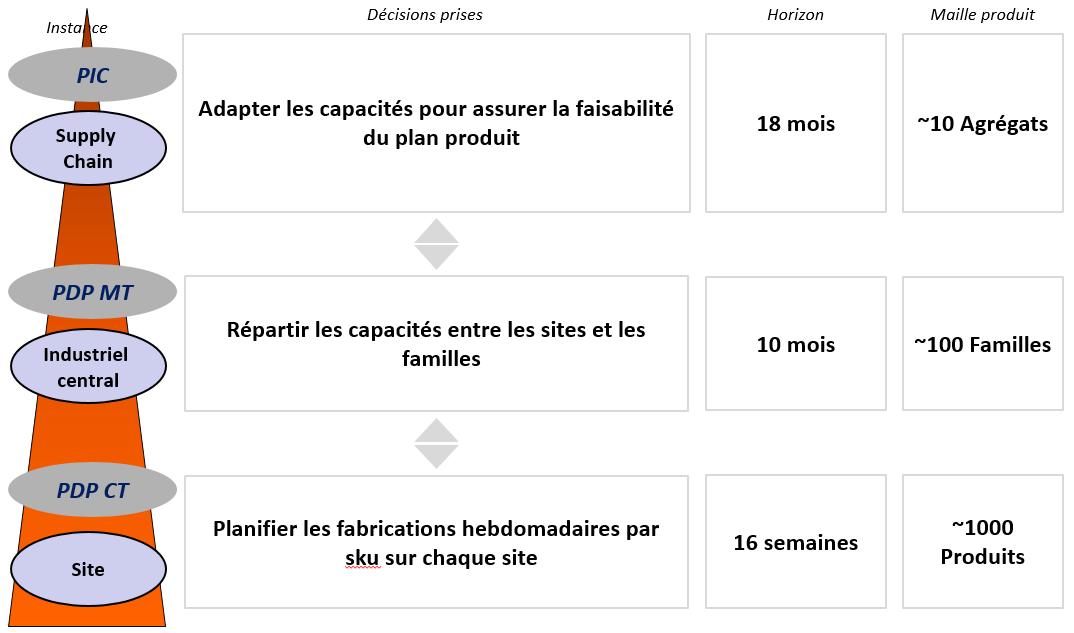
\includegraphics[width=\textwidth]{main/introduction/images/exemple_SC_luxe.png}
%   \caption{Exemple d'organisation de la Supply Chain d'un acteur du luxe}
%   \label{fig:exemple-SC-luxe}
% \end{figure}


% \section{Conséquences et problèmes étudiés}


% Optimsation multi-objectif : triangle coût / stock / service. (coût = coût hors stock).


% 2 sujets traités:
% \begin{itemize}
%   \item le niveau de multi-sourcing (moyen terme).
%   \begin{itemize}
%     \item Objectif : minimiser les coût de la création du multi-sourcing
%     \item Contrainte : taux de service client
%     \item Décisions : affectation produits / site
%   \end{itemize}
%   \item la plannification sous contrainte de flexibilité (court terme) décliné en deux axes :
%   \begin{itemize}
%     \item Optimization des paramètres des outils de PDP
%     \begin{itemize}
%       \item Objectif : minimiser le coût du stock
%       \item Contrainte : flexibilité industrielle (nombre de changements)
%       \item Décisions : Couverture de la production de chaque produits
%     \end{itemize}
%     \item Création du PDP en intégrant directement la contrainte de flexibilité
%     \begin{itemize}
%       \item Objectif : minimiser le coût du stock
%       \item Contrainte : flexibilité industrielle (nombre de changements)
%       \item Décisions : période de production et quantité produite pour chaque produit
%     \end{itemize}
%   \end{itemize}
% \end{itemize}


% Parler de la flexibilité du mix produit ! C'est ce qu'on optimise (ie : volume constant.)